\documentclass[11pt,a4paper]{article}

% ---------------------------------------------------------------
% Packages
% ---------------------------------------------------------------
\usepackage[utf8]{inputenc}
\usepackage[T1]{fontenc}
\usepackage{lmodern}
\usepackage[margin=2.2cm]{geometry}
\usepackage{xcolor}
\usepackage{amssymb}
\usepackage{enumitem}
\usepackage{booktabs}
\usepackage{tabularx}
\usepackage{array}
\usepackage{tikz}
\usetikzlibrary{arrows.meta, positioning, calc, shapes.geometric}
\usepackage{titlesec}
\usepackage[hidelinks]{hyperref}

% ---------------------------------------------------------------
% Colours and styles (same identity as the subject proposal)
% ---------------------------------------------------------------
\definecolor{salva}{HTML}{1F4E79}
\definecolor{accent}{HTML}{C9A227}
\definecolor{errorred}{HTML}{A12A2A}

\titleformat{\section}{\large\bfseries\color{salva}}{\thesection.}{0.6em}{}
\titleformat{\subsection}{\normalsize\bfseries\color{salva!85}}{\thesubsection}{0.6em}{}
\titlespacing*{\section}{0pt}{1.4em}{0.6em}
\titlespacing*{\subsection}{0pt}{1.0em}{0.4em}

\setlist{itemsep=0.2em, topsep=0.4em}
\setlength{\parindent}{0pt}
\setlength{\parskip}{0.5em}

\newcommand{\done}{\textcolor{salva}{\checkmark}}
\newcommand{\nd}[1]{\emph{#1}}             % an n8n node name
\newcommand{\st}[1]{\texttt{#1}}           % a request status
\newcolumntype{L}{>{\raggedright\arraybackslash}X}
% Tables stay where they are written (no floating): each one is a minipage, so it never
% splits from its caption. \tabcaption prints the numbered caption and closes the minipage.
\newcommand{\tabcaption}[1]{\par\vspace{0.4em}\refstepcounter{table}%
  {\normalsize Table~\thetable: #1\par}\end{minipage}\par\vspace{0.8em}}

% ---------------------------------------------------------------
% Document information -- edit these fields
% ---------------------------------------------------------------
\newcommand{\studentname}{[Your Name]}
\newcommand{\coursename}{[Course Name]}
\newcommand{\instructor}{[Instructor]}
\newcommand{\submissiondate}{\today}

\begin{document}

% ---------------------------------------------------------------
% Title block
% ---------------------------------------------------------------
\begin{center}
  {\small\scshape\color{salva!80} Final Project Report}\\[0.6em]
  {\LARGE\bfseries B2B Intelligent Order \& Inquiry Assistant}\\[0.3em]
  {\large for \textbf{Salva Import}}\\[1em]
  \begin{tabular}{@{}r@{\hspace{0.6em}}l@{}}
    \textbf{Student:}    & \studentname \\
    \textbf{Course:}     & \coursename \\
    \textbf{Instructor:} & \instructor \\
    \textbf{Date:}       & \submissiondate \\
  \end{tabular}
\end{center}

\vspace{0.4em}
{\color{salva}\hrule height 0.8pt}
\vspace{0.6em}

\textbf{Summary.} Salva Import sells Cumbé, a premium Colombian aguardiente, to bars,
restaurants and shops. This project delivers a Telegram assistant, built with n8n, that lets
these B2B clients ask product questions and place restock orders at any hour, in English, French
or Spanish. The assistant understands free text with Claude, answers product questions from the
brand's official content through a retrieval sub-workflow, checks and reserves live stock
through a REST API, sends a priced receipt, and hands the conversation to the sales team when
it cannot finish on its own. Every request is logged with a status. The system runs 24/7 on
Salva Import's server behind \url{https://bot.cumbespirits.fr}. It reaches the Level~3
(Advanced) target set in the subject proposal without using the planned cut line, and adds
six improvements beyond the original scope.

% ===============================================================
\section{Context and objective}
% ===============================================================
Salva Import's clients are professionals who restock between services, often outside office
hours. Before this project, every question (``What does Cumbé taste like?'') or order (``3 cases
of the 1~L'') had to wait for a sales representative to read an email.

\textbf{The need, in one sentence:} Salva Import's B2B clients need a way to instantly ask
questions about Cumbé and place restock orders at any hour, instead of waiting for business
hours to reach a sales representative.

The product range handled by the assistant is Cumbé Premium Aguardiente (29\% ABV, Pimpinella
anise, rested in Colombian oak casks) in 70~cl and 1~L bottles, sold by cases of 6.

% ===============================================================
\section{What the assistant does}
% ===============================================================
From the client's point of view, the assistant is a Telegram contact that:
\begin{itemize}
  \item \textbf{understands free text} in English, French and Spanish, and always replies in the
        client's language;
  \item \textbf{answers product questions} (tasting notes, serving, the four official cocktails)
        using only Salva Import's own content, and says so when it does not know;
  \item \textbf{takes orders}: it matches the product and bottle size, checks live stock,
        reserves the bottles and sends a receipt with unit price and total;
  \item \textbf{asks a clarifying question} when an order is incomplete (``70~cl or 1~L?'') and
        remembers the answer for 30~minutes, so ``1L'' is enough to complete the order;
  \item \textbf{escalates to a human}: if the inventory system is unavailable, the sales team is
        alerted in a private Telegram group and can chat with the client through the bot.
\end{itemize}

% ===============================================================
\section{Architecture}
% ===============================================================
\subsection{Infrastructure}

The solution runs as five Docker services on Salva Import's existing server (OVH VPS, Ubuntu,
4~vCPU, 7.6~GB RAM), next to the company website (Figure~\ref{fig:infra}).

\begin{figure}[htbp]
\centering
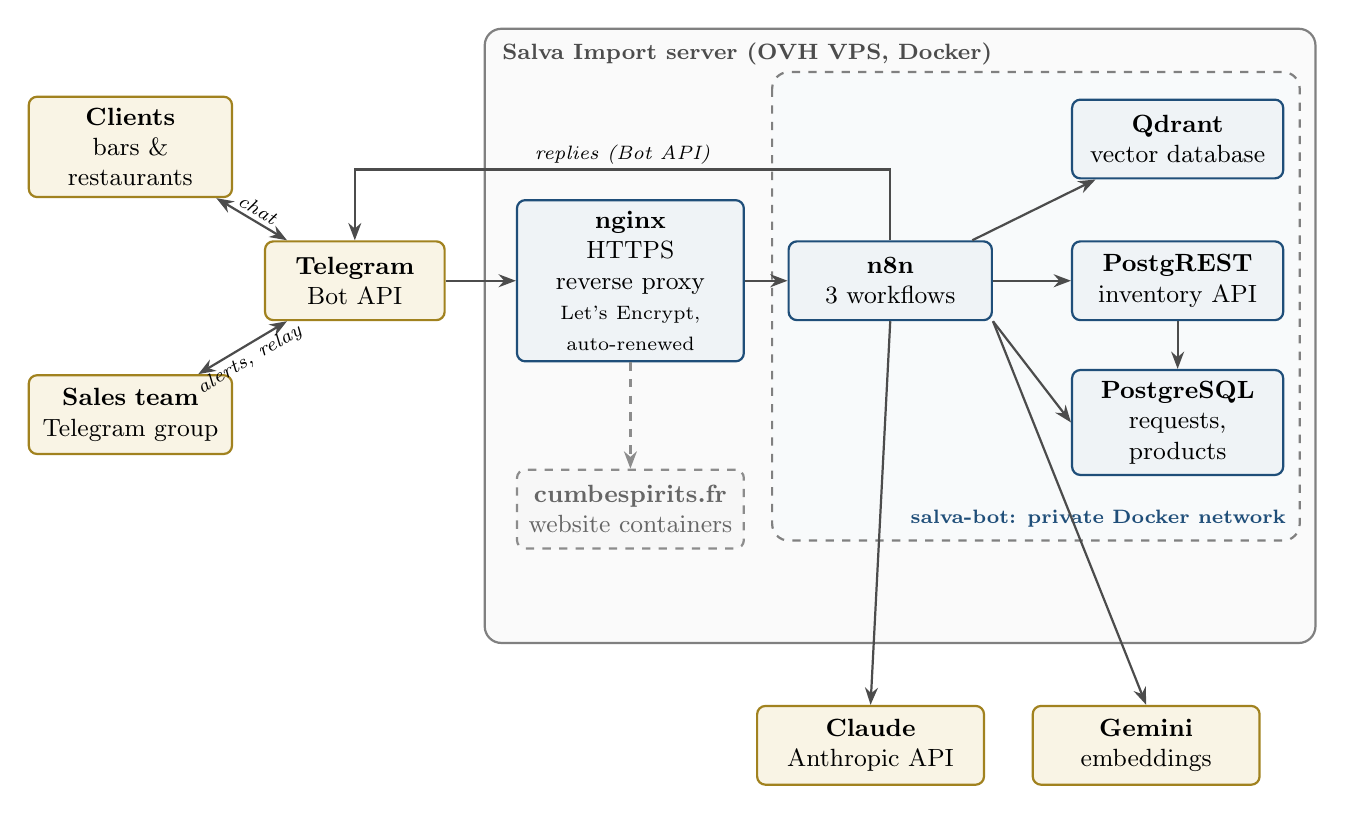
\begin{tikzpicture}[
  font=\small,
  box/.style={rectangle, rounded corners=3pt, draw=salva, thick, fill=salva!7, align=center,
              inner sep=4pt, minimum height=10mm, execute at begin node={\hyphenpenalty=10000}},
  ext/.style={box, draw=accent!80!black, fill=accent!12},
  ghost/.style={box, dashed, draw=black!45, fill=black!3, text=black!60},
  frame/.style={rounded corners=6pt, draw=black!50, thick},
  arrow/.style={-{Stealth[length=2.2mm]}, thick, draw=black!70},
  biarrow/.style={{Stealth[length=2.2mm]}-{Stealth[length=2.2mm]}, thick, draw=black!70},
  lbl/.style={font=\scriptsize\itshape, inner sep=1.5pt, align=center},
]
  % Frames: the server, and the bot's private Docker network inside it
  \draw[frame, fill=black!2] (4.5,1.5) rectangle (15.05,-6.3);
  \node[anchor=north west, font=\footnotesize\bfseries, text=black!70] at (4.6,1.45)
       {Salva Import server (OVH VPS, Docker)};
  \draw[frame, dashed, fill=salva!3] (8.15,0.95) rectangle (14.85,-5.0);
  \node[anchor=south east, font=\scriptsize\bfseries, text=salva] at (14.8,-4.95)
       {salva-bot: private Docker network};

  % Outside the server
  \node[ext, text width=2.3cm] (client) at (0,0)    {\textbf{Clients}\\bars \& restaurants};
  \node[ext, text width=2.3cm] (sales)  at (0,-3.4) {\textbf{Sales team}\\Telegram group};
  \node[ext, text width=2.0cm] (tg)     at (2.85,-1.7) {\textbf{Telegram}\\Bot API};

  % On the server
  \node[box, text width=2.6cm] (nginx) at (6.35,-1.7)
       {\textbf{nginx}\\HTTPS reverse proxy\\{\scriptsize Let's Encrypt, auto-renewed}};
  \node[ghost, text width=2.6cm] (site) at (6.35,-4.6) {\textbf{cumbespirits.fr}\\website containers};
  \node[box, text width=2.3cm] (n8n) at (9.65,-1.7) {\textbf{n8n}\\3 workflows};
  \node[box, text width=2.4cm] (qdrant) at (13.3,0.1)  {\textbf{Qdrant}\\vector database};
  \node[box, text width=2.4cm] (api)    at (13.3,-1.7) {\textbf{PostgREST}\\inventory API};
  \node[box, text width=2.4cm] (pg)     at (13.3,-3.5) {\textbf{PostgreSQL}\\requests, products};

  % External AI services
  \node[ext, text width=2.6cm] (claude) at (9.4,-7.6)  {\textbf{Claude}\\Anthropic API};
  \node[ext, text width=2.6cm] (gemini) at (12.9,-7.6) {\textbf{Gemini}\\embeddings};

  % Flows
  \draw[biarrow] (client) -- node[lbl, sloped, above] {chat} (tg);
  \draw[biarrow] (sales)  -- node[lbl, sloped, below] {alerts, relay} (tg);
  \draw[arrow] (tg) -- (nginx);
  \draw[arrow] (nginx) -- (n8n);
  \draw[arrow, dashed, black!45] (nginx) -- (site);
  \draw[arrow] (n8n.north) -- ++(0,0.9) -| node[lbl, above, pos=0.25] {replies (Bot API)} (tg.north);
  \draw[arrow] (n8n) -- (qdrant);
  \draw[arrow] (n8n) -- (api);
  \draw[arrow] (n8n.south east) -- (pg.west);
  \draw[arrow] (api) -- (pg);
  \draw[arrow] (n8n.south) -- (claude.north);
  \draw[arrow] (n8n.south east) -- (gemini.north);
\end{tikzpicture}
\caption{Infrastructure. Only nginx is reachable from the internet; the bot's services share a
private Docker network and are never exposed directly.}
\label{fig:infra}
\end{figure}

\begin{description}[leftmargin=0pt, itemsep=0.3em]
  \item[n8n] runs three workflows: \nd{Salva -- Main} (the assistant), \nd{Salva -- Product
        knowledge} (the retrieval sub-workflow) and \nd{Salva -- Load knowledge} (a one-off
        loader for the vector database).
  \item[PostgreSQL] stores every request with its status (\st{requests}) and the catalogue with
        prices and stock (\st{products}).
  \item[PostgREST] turns the \st{products} table into a REST API. It connects with a read-only
        role that can read products and call one stock-reservation function, nothing else.
  \item[Qdrant] holds the product knowledge as vectors (embeddings computed by Gemini).
  \item[nginx] is the website's existing gateway. The bot was added as one extra site,
        \url{bot.cumbespirits.fr}, without changing the website's configuration.
  \item[Claude] (Anthropic) reads every message and writes the answers to product questions.
\end{description}

\subsection{The main workflow}

Figure~\ref{fig:workflow} shows \nd{Salva -- Main} grouped into stages. Node names are in
italics, as they appear in n8n.

\begin{figure}[p]
\centering
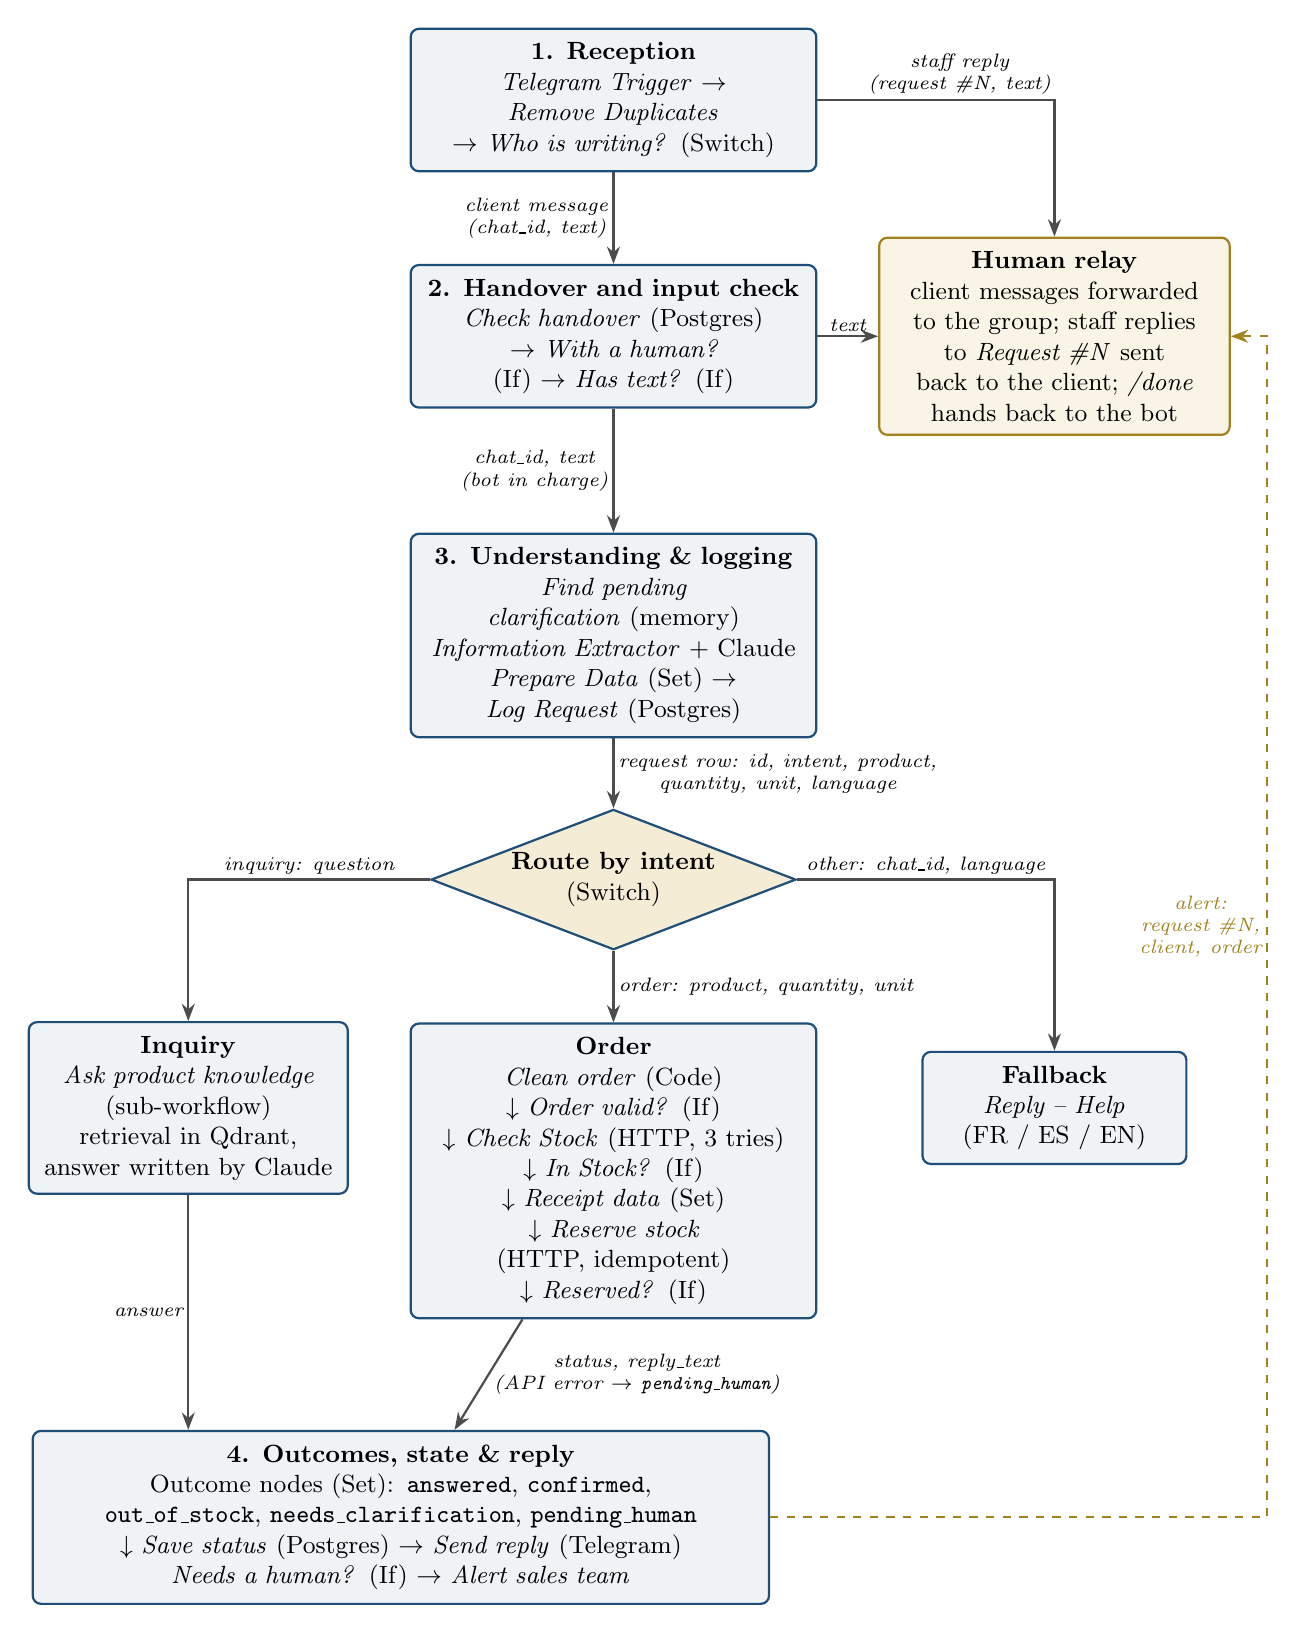
\begin{tikzpicture}[
  font=\small,
  stage/.style={rectangle, rounded corners=3pt, draw=salva, thick, fill=salva!7, align=center,
                inner sep=5pt, text width=4.8cm, execute at begin node={\hyphenpenalty=10000}},
  human/.style={stage, draw=accent!80!black, fill=accent!12},
  decision/.style={diamond, aspect=2.6, draw=salva, thick, fill=accent!20, align=center,
                   inner sep=1pt},
  arrow/.style={-{Stealth[length=2.2mm]}, thick, draw=black!70},
  lbl/.style={font=\scriptsize\itshape, inner sep=1.5pt, align=center},
]
  \node[stage] (recv) at (0,0)
       {\textbf{1. Reception}\\ \nd{Telegram Trigger} $\rightarrow$ \nd{Remove Duplicates}\\
        $\rightarrow$ \nd{Who is writing?} (Switch)};
  \node[stage] (hand) at (0,-3.0)
       {\textbf{2. Handover and input check}\\ \nd{Check handover} (Postgres) $\rightarrow$
        \nd{With a human?} (If) $\rightarrow$ \nd{Has text?} (If)};
  \node[human, text width=4.1cm] (relay) at (5.6,-3.0)
       {\textbf{Human relay}\\ client messages forwarded to the group; staff replies to
        \emph{Request \#N} sent back to the client; \emph{/done} hands back to the bot};
  \node[stage] (und) at (0,-6.8)
       {\textbf{3. Understanding \& logging}\\ \nd{Find pending clarification} (memory)\\
        \nd{Information Extractor} + Claude\\ \nd{Prepare Data} (Set) $\rightarrow$
        \nd{Log Request} (Postgres)};
  \node[decision] (route) at (0,-9.9) {\textbf{Route by intent}\\(Switch)};
  \node[stage, text width=3.7cm] (inq) at (-5.4,-12.8)
       {\textbf{Inquiry}\\ \nd{Ask product knowledge} (sub-workflow)\\ retrieval in Qdrant,
        answer written by Claude};
  \node[stage] (ord) at (0,-13.6)
       {\textbf{Order}\\ \nd{Clean order} (Code)\\ $\downarrow$ \nd{Order valid?} (If)\\
        $\downarrow$ \nd{Check Stock} (HTTP, 3 tries)\\ $\downarrow$ \nd{In Stock?} (If)\\
        $\downarrow$ \nd{Receipt data} (Set)\\ $\downarrow$ \nd{Reserve stock} (HTTP, idempotent)\\
        $\downarrow$ \nd{Reserved?} (If)};
  \node[stage, text width=3.0cm] (help) at (5.6,-12.8)
       {\textbf{Fallback}\\ \nd{Reply -- Help}\\ (FR / ES / EN)};
  \node[stage, text width=9.0cm] (out) at (-2.7,-18.0)
       {\textbf{4. Outcomes, state \& reply}\\ Outcome nodes (Set): \st{answered}, \st{confirmed},
        \st{out\_of\_stock}, \st{needs\_clarification}, \st{pending\_human}\\ $\downarrow$
        \nd{Save status} (Postgres) $\rightarrow$ \nd{Send reply} (Telegram)\\
        \nd{Needs a human?} (If) $\rightarrow$ \nd{Alert sales team}};

  \draw[arrow] (recv) -- node[lbl, left] {client message\\(chat\_id, text)} (hand);
  \draw[arrow] (recv.east) -| node[lbl, above, pos=0.3] {staff reply\\(request \#N, text)} (relay.north);
  \draw[arrow] (hand) -- node[lbl, above] {text} (relay);
  \draw[arrow] (hand) -- node[lbl, left] {chat\_id, text\\(bot in charge)} (und);
  \draw[arrow] (und) -- node[lbl, right] {request row: id, intent, product,\\quantity, unit, language} (route);
  \draw[arrow] (route.west) -| node[lbl, above, pos=0.25] {inquiry: question} (inq.north);
  \draw[arrow] (route) -- node[lbl, right] {order: product, quantity, unit} (ord);
  \draw[arrow] (route.east) -| node[lbl, above, pos=0.25] {other: chat\_id, language} (help.north);
  \draw[arrow] (inq.south) -- node[lbl, left] {answer} (inq.south |- out.north);
  \draw[arrow] (ord) -- node[lbl, right] {status, reply\_text\\(API error $\rightarrow$ \st{pending\_human})} (out);
  \draw[arrow, dashed, accent!80!black] (out.east) -- (8.3,-18.0) -- node[lbl, left, pos=0.5]
       {alert:\\request \#N,\\client, order} (8.3,-3.0) -- (relay.east);
\end{tikzpicture}
\caption{\nd{Salva -- Main}, grouped by stage, with the data carried by each arrow. Blue: automated
processing; gold: the human relay with the sales team. Messages without text, and any failure of
the AI node, go to \nd{Reply -- Usage}. Every external call retries 3 times, and any unexpected
failure starts \nd{Salva -- Error handler}, which posts the workflow name, error and execution
URL to the sales group.}
\label{fig:workflow}
\end{figure}

\paragraph{Reception and routing.} \nd{Who is writing?} separates private chats (clients)
from replies written by the sales team in their group; any other group message is ignored.
\nd{Check handover} then looks for a conversation currently handled by a salesperson (less
than two hours of silence). If there is one, the message is forwarded to the group instead of
being processed by the bot.

\paragraph{Understanding.} \nd{Find pending clarification} retrieves a question the bot asked
the same client in the last 30~minutes. The \nd{Information Extractor}, driven by Claude,
receives the message (or the earlier message, the question and the new answer) and returns
structured data: \st{intent} (\st{order}, \st{inquiry} or \st{other}), \st{product},
\st{quantity}, \st{unit} and \st{language}. \nd{Prepare Data} flattens this record, and
\nd{Log Request} stores it in PostgreSQL \emph{before} any further processing, so no request is
ever lost. \nd{Route by intent} has a fallback output: an unexpected classification goes to the
help message instead of disappearing.

\paragraph{Inquiry path (sub-workflow and vector database).} \nd{Ask product knowledge}
calls the sub-workflow \nd{Salva -- Product knowledge}, whose only input is the question and
whose only output is the answer. Inside, a Question-and-Answer chain retrieves the four closest
passages from Qdrant and lets Claude answer \emph{using only those passages}, in the language of
the question. The knowledge base contains the official Cumbé content: product facts, tasting
notes, serving advice and the four official cocktails (Guaro Sour, Feliz Endings, Pimpinella,
Carajillo). Prices and stock are deliberately absent from it: they change, so they stay in the
database.

\paragraph{Order path.} The AI is good at understanding language; exact business rules are
better handled by code. \nd{Clean order} (JavaScript) removes accents and capitals, matches
the product to a catalogue SKU, reads the bottle size from expressions such as ``1L'', ``70cl'' or
``0,7~l'', and validates the quantity. If something is missing it writes a short question in the
client's language. Otherwise \nd{Check Stock} reads the product from the inventory API,
\nd{In Stock?} compares bottles needed with bottles available, \nd{Receipt data} computes
the total, and \nd{Reserve stock} deducts the bottles through the API.

\paragraph{Outcomes, state and reply.} Each outcome is a Set node that produces the same four
fields (\st{request\_id}, \st{chat\_id}, \st{status}, \st{reply\_text}). This lets a single
\nd{Save status} node update the request in the database and a single \nd{Send reply} node
answer the client. For example, a confirmed order of 3 cases of Cumbé 1~L produces a receipt for
18 bottles at 153.00~EUR per case, total 459.00~EUR excl.~VAT, formatted in the client's language.

\paragraph{Human in the loop.} When a request ends in \st{pending\_human}, \nd{Alert sales
team} posts it in the private group. A salesperson answers by replying to the alert; the bot
delivers the reply to the client and marks the request \st{handled\_by\_human}. The client's
next messages are relayed to the group until a salesperson replies \emph{/done} or two hours pass
without activity.

\subsection{Data model and request lifecycle}

\par\noindent\begin{minipage}{\linewidth}
\centering\small
\renewcommand{\arraystretch}{1.25}
\begin{tabularx}{\linewidth}{@{}l L@{}}
  \toprule
  \textbf{Table / columns} & \textbf{Purpose} \\
  \midrule
  \multicolumn{2}{@{}l}{\textbf{\st{requests}}: one row per incoming client message} \\
  \st{id}, \st{created\_at}, \st{chat\_id}, \st{client\_name}, \st{message} & who wrote what, and when \\
  \st{intent}, \st{product}, \st{quantity}, \st{unit}, \st{language} & what the AI understood \\
  \st{status}, \st{bot\_reply} & the outcome and what the bot answered \\
  \st{follow\_up\_of} & links a short answer to the question it completes \\
  \st{reserved\_sku}, \st{reserved\_bottles} & stock reserved for this request \\
  \st{human\_last\_at} & last activity in a conversation handled by a salesperson \\
  \midrule
  \multicolumn{2}{@{}l}{\textbf{\st{products}}: the catalogue} \\
  \st{sku}, \st{name}, \st{category}, \st{bottle\_ml} & product identity and format \\
  \st{bottles\_per\_case}, \st{price\_per\_case}, \st{stock\_bottles} & ordering unit, price, live stock \\
  \bottomrule
\end{tabularx}
\tabcaption{PostgreSQL tables. \st{chat\_id} is a \st{BIGINT}: Telegram identifiers exceed the
range of a standard integer.}

\begin{figure}[htbp]
\centering
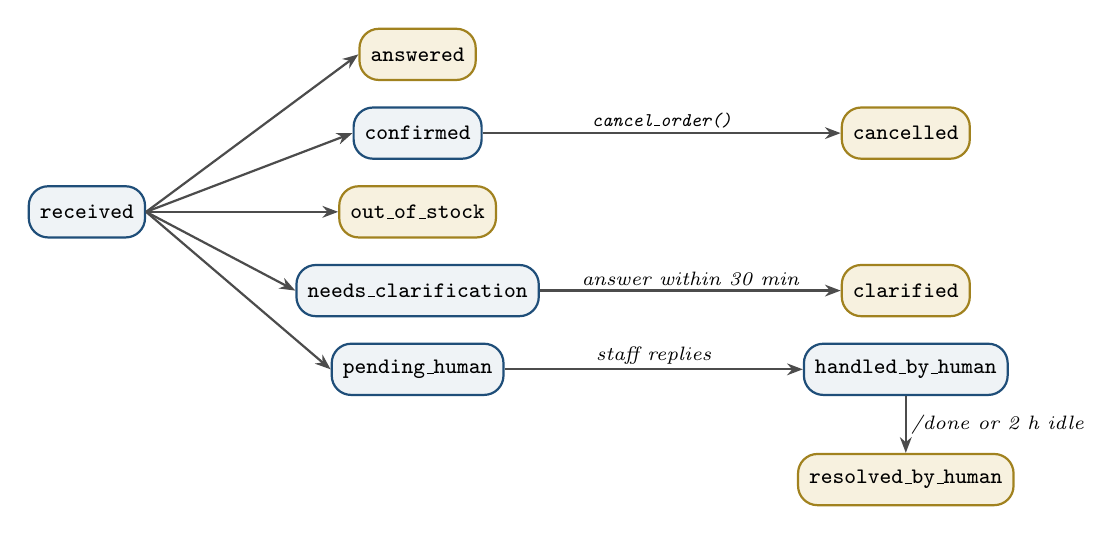
\begin{tikzpicture}[
  font=\small,
  st/.style={rectangle, rounded corners=7pt, draw=salva, thick, fill=salva!7,
             font=\ttfamily\footnotesize, inner sep=4pt, minimum height=6.5mm},
  fin/.style={st, draw=accent!80!black, fill=accent!15},
  arrow/.style={-{Stealth[length=2mm]}, thick, draw=black!70},
  lbl/.style={font=\scriptsize\itshape, inner sep=1.5pt},
]
  \node[st]  (rec)  at (0,0)      {received};
  \node[fin] (ans)  at (4.2,2.0)  {answered};
  \node[st]  (conf) at (4.2,1.0)  {confirmed};
  \node[fin] (oos)  at (4.2,0)    {out\_of\_stock};
  \node[st]  (nc)   at (4.2,-1.0) {needs\_clarification};
  \node[st]  (ph)   at (4.2,-2.0) {pending\_human};
  \node[fin] (can)  at (10.4,1.0)  {cancelled};
  \node[fin] (cla)  at (10.4,-1.0) {clarified};
  \node[st]  (hbh)  at (10.4,-2.0) {handled\_by\_human};
  \node[fin] (rbh)  at (10.4,-3.4) {resolved\_by\_human};

  \foreach \t in {ans, conf, oos, nc, ph} \draw[arrow] (rec.east) -- (\t.west);
  \draw[arrow] (conf) -- node[lbl, above] {\texttt{cancel\_order()}} (can);
  \draw[arrow] (nc)   -- node[lbl, above] {answer within 30 min} (cla);
  \draw[arrow] (ph)   -- node[lbl, above] {staff replies} (hbh);
  \draw[arrow] (hbh)  -- node[lbl, right] {/done or 2 h idle} (rbh);
\end{tikzpicture}
\caption{Request statuses. Gold boxes are final states. Greetings and off-topic messages receive
the help message and keep the status \st{received}.}
\label{fig:lifecycle}
\end{figure}

% ===============================================================
\section{Minimum technical requirements}
% ===============================================================
\par\noindent\begin{minipage}{\linewidth}
\centering\small
\renewcommand{\arraystretch}{1.3}
\begin{tabularx}{\linewidth}{@{}c l L@{}}
  \toprule
   & \textbf{Requirement} & \textbf{Where it is in the project} \\
  \midrule
  \done & Message trigger & \nd{Telegram Trigger}, reached over HTTPS at \url{bot.cumbespirits.fr} \\
  \done & AI node & \nd{Information Extractor} with Claude (intent, product, quantity, unit,
                     language); Question-and-Answer chain in the sub-workflow \\
  \done & Router / If / Switch & \nd{Who is writing?} and \nd{Route by intent} (Switch, with
                                 fallback); \nd{With a human?}, \nd{Order valid?},
                                 \nd{In Stock?}, \nd{Reserved?}, \nd{Needs a human?} (If) \\
  \done & If or Set node & \nd{Prepare Data}, \nd{Receipt data} and the Outcome nodes, which
                           format the receipt and every reply \\
  \done & Code node & \nd{Clean order}: SKU matching, bottle-size parsing, quantity validation,
                      multilingual questions \\
  \done & API connection & \nd{Check Stock} and \nd{Reserve stock}: HTTP calls to the PostgREST
                           inventory API \\
  \done & Database & PostgreSQL (requests with status, catalogue) and Qdrant (vector database) \\
  \done & Sub-workflow & \nd{Salva -- Product knowledge}, called by \nd{Ask product knowledge} \\
  \done & Error handling and retries & Retry On Fail (3 attempts, 2~s apart) on every AI,
                                       database, HTTP and Telegram node; API errors end in
                                       \st{pending\_human} with a polite message and a sales alert;
                                       AI errors and messages without text get a usage message;
                                       \nd{Salva -- Error handler} (Error Trigger) alerts the sales
                                       group with the workflow name and execution URL \\
  \bottomrule
\end{tabularx}
\tabcaption{Course requirements and the nodes that implement them.}

% ===============================================================
\section{Reliability, safety and security}
% ===============================================================
\begin{itemize}
  \item \textbf{No silent failures.} Both Switch nodes have explicit handling for unexpected
        input; Postgres look-ups that may return nothing use \emph{Always Output Data}; every
        external call has retries; API calls and the AI node have an error output; an Error
        Workflow reports any other failure with a link to the execution.
  \item \textbf{No duplicates.} \nd{Remove Duplicates} drops a Telegram update that was already
        processed (same \st{update\_id}), so a message delivered twice creates no second row and
        no second reply.
  \item \textbf{No overselling.} Reservation is a single database operation that only succeeds if
        enough bottles remain; PostgreSQL locks the product row while it runs:
\end{itemize}
\begin{minipage}{\linewidth}
\small
\begin{verbatim}
    UPDATE products
       SET stock_bottles = stock_bottles - p_bottles
     WHERE sku = p_sku AND p_bottles > 0 AND stock_bottles >= p_bottles
    RETURNING stock_bottles;
\end{verbatim}
\end{minipage}
\begin{itemize}
  \item \textbf{Safe retries (idempotency).} The function \st{reserve\_stock} first checks whether
        the request already holds a reservation. A retried call therefore never deducts the same
        order twice. \st{cancel\_order} gives the bottles back.
  \item \textbf{Least privilege.} The inventory API cannot modify the catalogue directly and
        cannot read client data: its role may only read \st{products} and call
        \st{reserve\_stock}.
  \item \textbf{Isolation.} The database, the API and Qdrant listen only on the private Docker
        network or on the server's loopback interface. nginx resolves the bot only when a request
        arrives, so the website keeps working even if the bot is stopped.
  \item \textbf{Transport and access.} HTTPS with Let's Encrypt certificates renewed and installed
        automatically; two-factor authentication on the n8n account; secrets kept in a
        server-side \st{.env} file and never exported with the workflows.
\end{itemize}

% ===============================================================
\section{Deployment and operations}
% ===============================================================
The project was first built on a laptop, then moved to the company server as a Docker Compose
project (\st{salva-bot}). The migration copied the three data volumes (n8n, PostgreSQL, Qdrant),
so workflows, encrypted credentials, logged requests and vectors moved unchanged. The tunnel used
during development (ngrok) was replaced by an extra site in the website's existing nginx, with its
own certificate. During this work, a misconfiguration in the \emph{website's} certificate renewal
was found and fixed: it would have caused a certificate error on \url{cumbespirits.fr} in
November.

The project is versioned in a Git repository: Compose file with every image pinned to an exact
version and digest, \st{.env.example} (the real \st{.env}, which also holds
\st{N8N\_ENCRYPTION\_KEY}, is git-ignored), database init scripts that rebuild the full schema and
the API roles on a fresh volume, the workflows exported as JSON, and a README describing setup
from a fresh clone, the environment variables and the tests.

\par\noindent\begin{minipage}{\linewidth}
\centering\small
\renewcommand{\arraystretch}{1.25}
\begin{tabularx}{\linewidth}{@{}l L@{}}
  \toprule
  \textbf{Task} & \textbf{How} \\
  \midrule
  Check the services & \texttt{docker compose ps} in \texttt{\textasciitilde/salva-bot} \\
  Follow a run & n8n \emph{Executions} tab, or \texttt{docker compose logs n8n} \\
  Back up the database & \texttt{pg\_dump} through \texttt{docker compose exec postgres} \\
  Cancel an order & \texttt{SELECT cancel\_order(N);} (releases the reserved bottles) \\
  Reserve stock for a manually confirmed order & \texttt{SELECT reserve\_stock(N, 'SKU', bottles);} \\
  Update the product knowledge & delete the Qdrant collection, then run \nd{Salva -- Load knowledge} \\
  Certificates & renewed by certbot; deploy hooks copy them to nginx and reload it \\
  \bottomrule
\end{tabularx}
\tabcaption{Day-to-day operations.}

% ===============================================================
\section{Testing and demonstration}
% ===============================================================
\par\noindent\begin{minipage}{\linewidth}
\centering\small
\renewcommand{\arraystretch}{1.3}
\begin{tabularx}{\linewidth}{@{}c L L@{}}
  \toprule
  \textbf{\#} & \textbf{Client message or action} & \textbf{Expected behaviour} \\
  \midrule
  1 & ``Bonjour'' & help message in French (fallback path) \\
  2 & ``Quel cocktail faire avec du café ?'' & the Carajillo recipe, in French (sub-workflow and
                                               vector database) \\
  3 & ``I need 3 cases of Cumbé 1L'' & receipt: 18 bottles, 459.00~EUR excl.~VAT; stock reduced by 18 \\
  4 & ``Je veux 4 caisses de Cumbé'', then ``70 cl'' & ``70~cl or 1~L?'', then a receipt for 4 cases
                                                     of 70~cl (memory) \\
  5 & ``Quiero 50 cajas de Cumbé 70cl'' & out-of-stock answer in Spanish \\
  6 & inventory API stopped, then an order & ``system busy'' message, alert in the sales group,
                                             status \st{pending\_human} \\
  7 & salesperson replies to the alert; client answers; salesperson sends \emph{/done} &
      two-way conversation through the bot; bot back in charge afterwards \\
  8 & the same reservation sent twice & second call returns \st{already\_reserved}; stock
                                        unchanged \\
  9 & the pinned test message executed twice & second run stops at \nd{Remove Duplicates}: no row,
                                                no message \\
  10 & a sticker instead of text & usage message in the client's language \\
  11 & \url{bot.cumbespirits.fr/webhook/error-test} & the Error Workflow alerts the sales group with
                                                      the execution link \\
  \bottomrule
\end{tabularx}
\tabcaption{Test and demonstration scenarios, all run end to end from a phone.}

% ===============================================================
\section{From the proposal to the final product}
% ===============================================================
The subject proposal targeted Level~3 (Advanced), with a cut line that would have removed the
inventory API and the vector database if time ran short. \textbf{The cut line was not needed}: both
components are in production. Table~\ref{tab:upgrades} lists the six improvements that go
beyond the proposal.

\par\noindent\begin{minipage}{\linewidth}
\centering\small
\renewcommand{\arraystretch}{1.25}
\begin{tabularx}{\linewidth}{@{}l L@{}}
  \toprule
  \textbf{Upgrade} & \textbf{Result} \\
  \midrule
  Server deployment & runs 24/7 on the company server at \url{bot.cumbespirits.fr}, with HTTPS \\
  Conversation memory & a short answer (``1L'', ``6'') completes the previous order \\
  Stock reservation & atomic and idempotent; orders can be cancelled \\
  Sales team alerts & \st{pending\_human} requests are posted in a private Telegram group \\
  Two-way relay & salespeople and clients chat through the bot; \emph{/done} hands back \\
  Multilingual replies & every message, including clarifying questions, in EN / FR / ES \\
  \bottomrule
\end{tabularx}
\tabcaption{Improvements delivered beyond the subject proposal.\label{tab:upgrades}}

% ===============================================================
\section{Challenges and lessons learned}
% ===============================================================
\par\noindent\begin{minipage}{\linewidth}
\centering\small
\renewcommand{\arraystretch}{1.25}
\begin{tabularx}{\linewidth}{@{}>{\raggedright\arraybackslash}p{4.1cm} L L@{}}
  \toprule
  \textbf{Symptom} & \textbf{Cause} & \textbf{Lesson} \\
  \midrule
  Telegram error ``chat not found'' & a field in \emph{Fixed} mode sent the expression as plain text
    & an expression field must show the \emph{fx} badge and a real preview value \\
  ``Referenced node doesn't exist'' & node names in \texttt{\$('...')} are case-sensitive
    & drag fields from the input panel so n8n writes the exact name \\
  Every order reported ``out of stock'' & the API's JSON variant was not recognised, so the reply
    was kept as plain text & force \emph{Response Format: JSON} on HTTP nodes \\
  Receipt showed ``NaN'' & a field named \texttt{unit price} instead of \texttt{unit\_price}
    & consistent field names matter as much as the logic \\
  Bot stopped answering after a test & Telegram allows one webhook per bot; a manual test took it
    & test the live bot from a phone and follow runs in \emph{Executions} \\
  Workflow stopped without error & a database look-up returned no rows
    & use \emph{Always Output Data} on optional look-ups \\
  Database started without tables & a missing file was mounted, so Docker created a folder instead
    & check files exist before mounting them \\
  Telegram IDs rejected & identifiers larger than a 32-bit integer & use \texttt{BIGINT} \\
  Ports 80/443 already in use on the server & the website's nginx owns them
    & integrate with the existing gateway instead of adding a second one \\
  \bottomrule
\end{tabularx}
\tabcaption{Problems met while building the project, and what they taught.}

% ===============================================================
\section{Limitations and next steps}
% ===============================================================
\begin{itemize}
  \item \textbf{Relayed conversations are not stored.} The sales group serves as their history;
        saving them in the database would allow reporting.
  \item \textbf{Photos and voice messages} are announced to the sales team but not forwarded.
  \item \textbf{The product dictionary} used by \nd{Clean order} duplicates the catalogue; it
        could be generated from the \st{products} table so new products need no code change.
  \item \textbf{Free-form product chat} has no memory beyond order clarifications; a full chat
        memory would allow follow-up questions such as ``and the 1~L?''.
  \item \textbf{Personal data.} Client first names, Telegram identifiers and messages are stored;
        a retention period should be defined and applied (GDPR).
  \item \textbf{Single server.} Backups are manual; scheduled database backups and monitoring of
        the services would make the system production-grade.
\end{itemize}

\end{document}
